\documentclass[../../../include/open-logic-section]{subfiles}

\begin{document}

\olfileid[tr]{sth}{ordinals}{idea}	
\olsection{Sıra Sayısının Genel Fikri}

Doğal sayıları alışılmış sıraları içinde ele alın:
\begin{center}
	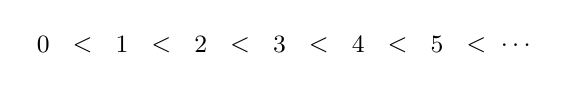
\begin{tikzpicture}
	\foreach \x/\xtext in {0, 1, 2, 3, 4, 5}
	{
		\node (\x a) at (\x, 1) {\small{$\x$}};
		\node (\x a) at (\x.5, 1) {\small{$<$}};
	}
	\node (ldots) at (6, 1) {\small{$\ldots$}};
	\end{tikzpicture}
\end{center}
Terminolojide buna bir $\omega$-dizisi denir. Gerçekten de bu genel
sıralama, küme hiyerarşisinin aşamalarına ilişkin ilk kuruluşumuzda
yansıtılır. Şimdi $0$'ı bu dizinin sonuna taşıdığımızı, yani bütün öteki
sayılardan sonra geldiğini varsayın:
\begin{center}
	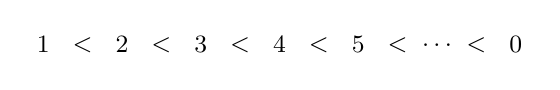
\begin{tikzpicture}
	\foreach \x/\xtext in {1, 2, 3, 4, 5}
	{
		\node (\x a) at (\x, 1) {\small{$\x$}};
		\node (\x a) at (\x.5, 1) {\small{$<$}};
	}
	\node (ldots) at (6, 1) {\small{$\ldots$}};
	\node (bea) at (6.5, 1) {\small{$<$}};
	\node (noa) at (7, 1) {\small{$0$}};
	\end{tikzpicture}
\end{center}
Burada aynı varlıklar vardır, fakat temelden farklı bir biçimde
sıralanmışlardır: ilk sıralamamızda son eleman yoktu, yeni sıralamamızdaysa
vardır. Gerçekten yeni sıralamamız, bir $\omega$-varlık dizisinin
($1,2,3,4,5,\ldots$) ardından başka bir varlığın gelmesinden oluşur. Bu
bir $\omega+1$-dizisidir.

Yalnızca bu varlıkları kullanarak daha fazla sıralama türü üretebiliriz.
Örneğin bütün çift sayıların (doğal sıralarında) ardından bütün tek
sayıların (doğal sıralarında) geldiğini düşünün:
\begin{center}
	\begin{tikzpicture}
	\node(a1) at (1,1) {\small{$0$}};
	\node(a2) at (1.5,1) {\small{$<$}};
	\node(a3) at (2,1) {\small{$2$}};
	\node(a4) at (2.5,1) {\small{$<$}};
	\node(a5) at (3,1) {\small{$4$}};
	\node(a6) at (3.5,1) {\small{$<$}};
	\node(dots) at (4,1) {\small{$\ldots$}};
	\node(aaoe) at (4.5,1) {\small{$<$}};
	\node(b1) at (5,1) {\small{$1$}};
	\node(b2) at (5.5,1) {\small{$<$}};
	\node(b3) at (6,1) {\small{$3$}};
	\node(b4) at (6.5,1) {\small{$<$}};
	\node(b5) at (7,1) {\small{$\ldots$}};
	\end{tikzpicture}
\end{center}
Bu, bir başka $\omega$-dizisinin izlediği bir $\omega$-dizisidir; yani
bir $\omega+\omega$-dizisi.

Bu biçimde ilerlemeyi sürdürebiliriz. Ancak istediğimiz şey,
\emph{sıralamalar} hakkındaki bu konuşmayı anlamanın genel bir yoludur.

\end{document}
